\documentclass[conference,a4paper]{IEEEtran}
\IEEEoverridecommandlockouts
\usepackage{cite}
\usepackage{amsmath,amssymb,amsfonts}
\usepackage{graphicx}
\usepackage{textcomp}
\usepackage{xcolor}
\usepackage{booktabs}
\usepackage{url}
\graphicspath{{../diagrams/}}

\begin{document}

\title{Agent Reliability Lab: Controlled Fault Injection and Evidence-Based Failure Analysis for Tool-Using Language Agents}

\author{\IEEEauthorblockN{Suryansh Singh}
\IEEEauthorblockA{\textit{Department of Computer Science and Engineering}\\
\textit{Noida Institute of Engineering and Technology}\\
Greater Noida, India\\
0231cse087@niet.co.in}
\and
\IEEEauthorblockN{Simran Kumari}
\IEEEauthorblockA{\textit{Department of Computer Science and Engineering}\\
\textit{Noida Institute of Engineering and Technology}\\
Greater Noida, India\\
0231cse179@niet.co.in}
\and
\IEEEauthorblockN{Tanishka Sahu}
\IEEEauthorblockA{\textit{Department of Computer Science and Engineering}\\
\textit{Noida Institute of Engineering and Technology}\\
Greater Noida, India\\
0231cse196@niet.co.in}
}

\maketitle

\begin{abstract}
Tool-using agents built on large language models plan, call external tools, read
observations, and retry after errors. Most evaluations still report a single success
rate from one attempt per task in a clean environment, which hides why runs fail, how
consistently an agent succeeds, and what reliability costs. This paper presents Agent
Reliability Lab, an open-source Python laboratory for controlled reliability
experiments on any agent that maps a task to a recorded trajectory. The laboratory
injects tool timeouts and outages on a seeded schedule that depends only on the task,
trial, tool, and call number, so every agent variant meets exactly the same failures and
their runs can be compared as matched pairs. It runs each task several times and
reports success with confidence intervals, the probability that all attempts succeed,
consistency, cost, latency, recovery, and step use. A rule-based classifier explains
each failed run as a planning, tool-misuse, context, recovery, or horizon failure with
evidence, and leaves unmatched failures unclassified. A configuration search returns the
cheapest setting that meets a reliability target. In preliminary experiments with
offline reference agents on a twelve-task customer-support suite, the measured effect of
injected faults matches the closed-form expectation, the classifier recovers every
planted defect with perfect precision, and the search identifies a retry budget that
keeps success above ninety-five percent under thirty percent tool timeouts.
\end{abstract}

\begin{IEEEkeywords}
agent evaluation, fault injection, failure analysis, reliability, tool use, large language models
\end{IEEEkeywords}

\section{Introduction}

Large language model (LLM) agents no longer answer a single prompt. Following the
reasoning and acting pattern of ReAct~\cite{yao2023react}, they decompose a goal, call
tools, read the results, and continue for many steps. Benchmarks such as
AgentBench~\cite{liu2024agentbench}, GAIA~\cite{mialon2024gaia},
SWE-bench~\cite{jimenez2024swebench}, WebArena~\cite{zhou2024webarena}, and
$\tau$-bench~\cite{yao2024taubench} have made agent capability measurable. They mostly
answer one question: did the agent finish the task?

Deployed agents face a harder question: will the agent finish the task every time, in a
world where tools time out, and at what cost? A single success rate cannot answer it.
Two agents with the same score may fail for unrelated reasons, one by guessing instead
of calling a required tool and another by abandoning a task after one timeout. Success
measured once per task also hides inconsistency; on $\tau$-bench the chance that a
strong model solves the same retail task in all of eight attempts falls below 25\% even
though its single-attempt success exceeds 60\%~\cite{yao2024taubench}. Kapoor
\textit{et al.} further showed that ignoring cost leads to needlessly complex agents and
mistaken conclusions about where accuracy gains come from~\cite{kapoor2024agents}.

This paper describes Agent Reliability Lab (relai), a laboratory in which these
questions become controlled experiments. Its contributions are:

\begin{enumerate}
\item A small agent interface, a name plus a run method that returns a trajectory, which
admits scripted policies, hand-written agents, and LLM agents behind any
OpenAI-compatible endpoint without changing the harness.
\item Seeded, agent-independent fault injection: each tool call fails or succeeds as a
deterministic function of the seed, task, trial, tool, and call number. All variants
meet the same failure schedule, which makes paired significance tests valid.
\item Repeated-trial reliability metrics with uncertainty: pass@$k$, pass$^k$,
consistency, Wilson and task-clustered bootstrap intervals, and an exact McNemar test
between variants.
\item An evidence-producing failure taxonomy with five modes and an explicit
unclassified outcome, validated against reference agents whose defects are planted on
purpose.
\item Cost- and latency-aware configuration search that returns the Pareto front and the
cheapest setting that meets a reliability target.
\end{enumerate}

Section~II reviews related work, Section~III states the problem, Section~IV describes
the methodology, Section~V reports preliminary results, and Section~VI concludes.

\section{Related Work}

\subsection{Agent Benchmarks and Reliability Metrics}
AgentBench~\cite{liu2024agentbench}, GAIA~\cite{mialon2024gaia},
SWE-bench~\cite{jimenez2024swebench}, and WebArena~\cite{zhou2024webarena} contribute
tasks and environments, and report task success. $\tau$-bench~\cite{yao2024taubench}
introduced pass$^k$, the chance that all of $k$ independent trials succeed, which
complements the pass@$k$ estimator of Chen \textit{et al.}~\cite{chen2021codex}; its
successor $\tau^2$-bench adds dual-control
environments~\cite{barres2025tau2}. The Holistic Agent Leaderboard (HAL) standardizes
cost-aware evaluation across benchmarks and uses LLM-aided log
inspection~\cite{kapoor2026hal}, and Rabanser \textit{et al.} decompose reliability
into consistency, robustness, predictability, and safety with twelve
metrics~\cite{rabanser2026reliability}. Agent Reliability Lab adopts pass$^k$ and cost
awareness from this line of work and adds paired statistical comparison and per-run
diagnosis.

\subsection{Fault Injection}
Chaos engineering deliberately injects failures into production systems to build
confidence in their resilience~\cite{basiri2016chaos}. For agents,
ToolEmu emulates tools with an LLM to expose risky behavior~\cite{ruan2024toolemu},
ToolMisuseBench offers replayable tool faults under call and retry
budgets~\cite{toolmisusebench2026}, ToolBench-X injects recoverable tool-environment
hazards~\cite{toolbenchx2026}, and AgentChaos injects faults into LLM API responses
through a proxy~\cite{agentchaos2026}. These works are benchmarks or injection layers.
Agent Reliability Lab treats the fault schedule as a controlled experimental factor that
is identical across variants and checks the injector against its analytic expectation.

\subsection{Failure Taxonomies and Attribution}
MAST derives fourteen failure modes for multi-agent systems from annotated
traces~\cite{cemri2025mast}, TRAIL annotates errors in long agent
traces~\cite{deshpande2025trail}, and Who\&When attributes failures to a responsible
agent and step~\cite{zhang2025whowhen}. These efforts rely on human annotation or LLM
judges, and the best automated attribution identifies the failing step in only 14.2\%
of cases~\cite{zhang2025whowhen}. Agent Reliability Lab uses deterministic rules over
structured trajectories, reports the evidence behind each label, and refuses to label
what no rule explains.

\subsection{Evaluation Frameworks}
General frameworks such as HELM~\cite{liang2023helm}, Inspect~\cite{inspect2024}, and
tracing platforms such as LangSmith and Langfuse record and score runs at scale.
They are complementary: Agent Reliability Lab is a small library for controlled
experiments that can run on a laptop with no model access.

\section{Problem Statement}

Let $\mathcal{T}$ be a suite of tasks, each with a prompt, an expected answer, a set of
permitted tools, and an optional step budget $B_t$. Let $\mathcal{V}$ be a set of agent
variants, such as different models, prompts, or retry policies. An environment exposes
tools whose calls may fail according to a fault process $F$ with seed $s$. Running
variant $v$ on task $t$ in trial $i$ produces a trajectory $\pi_{v,t,i}$: an ordered
sequence of plan, tool call, observation, error, recovery, and final steps, each with
optional latency, token, and cost annotations.

The problem is to design a laboratory that, for every $v \in \mathcal{V}$:
\begin{enumerate}
\item estimates success, pass$^k$, consistency, cost, latency, recovery, and step use
with honest uncertainty;
\item explains each failed run by a root cause with evidence, without forcing
unexplained failures into a category;
\item decides whether two variants differ significantly under identical faults; and
\item selects the configuration that minimizes cost subject to a reliability target.
\end{enumerate}
Any callable that maps a task to a trajectory must be admissible, and scoring and
analysis must read trajectories only, so that every number can be reproduced from
stored runs.

\section{Proposed Methodology}

Fig.~\ref{fig:architecture} shows the architecture. Inputs are a task suite and an
agent. The harness runs every variant on every task for $k$ trials, routing tool calls
through a fault-injecting environment. Scorers, metric derivation, and the failure
classifier read the finished trajectories. Statistics, optimization, storage, and
reporting operate on the resulting reports.

\begin{figure*}[t]
\centering
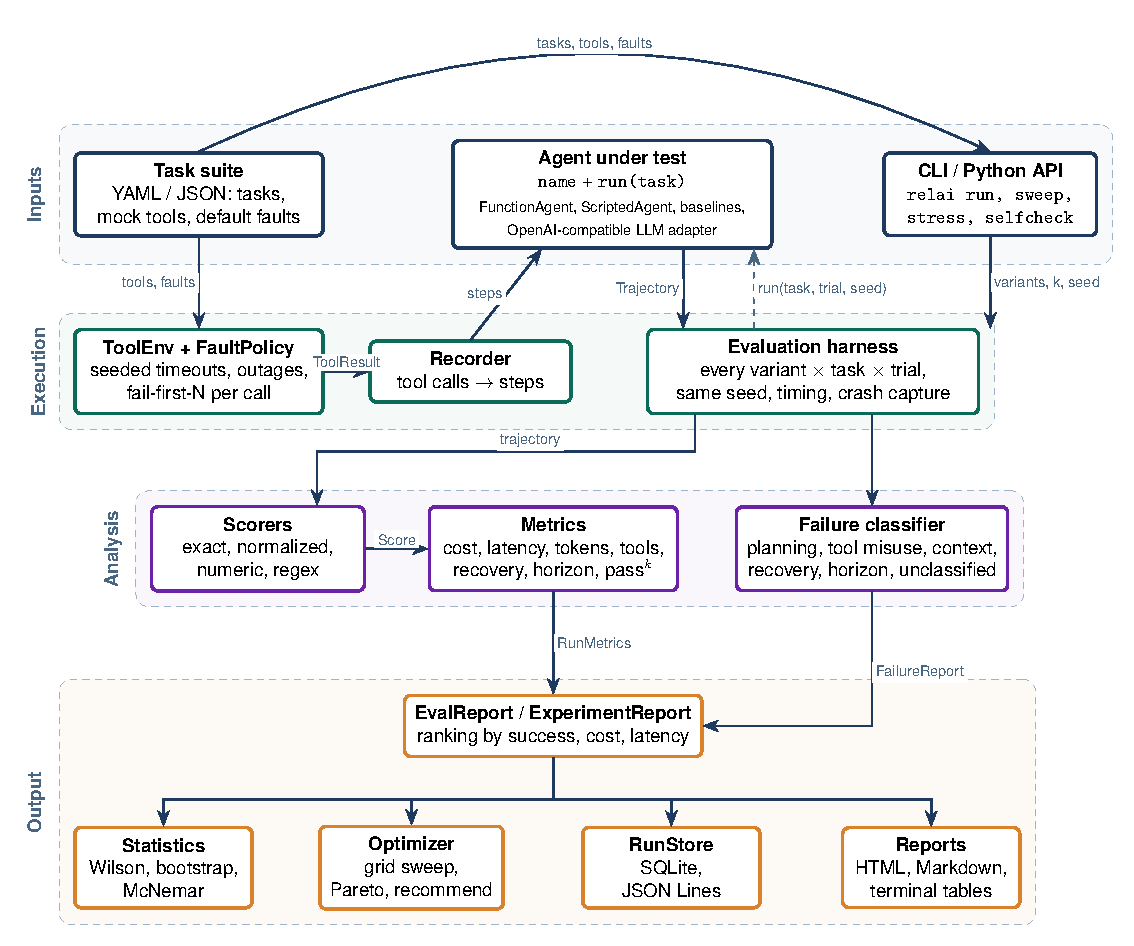
\includegraphics[width=0.86\textwidth]{architecture.pdf}
\caption{Architecture of Agent Reliability Lab. Only the execution layer calls agents;
every later layer reads recorded trajectories.}
\label{fig:architecture}
\end{figure*}

\subsection{Trajectory Model and Agent Interface}
A trajectory is a list of typed steps. Tool-call steps carry the tool name, arguments,
and an ok flag; an error step that follows a failed call marks an environment fault.
An agent needs only a name and a run method. Adapters wrap plain functions, replay
scripted trajectories, or drive an LLM through an OpenAI-compatible chat API, where a
recorder converts every model turn and tool call into steps with token, cost, and
latency annotations. Exceptions raised by an agent become failed runs, so one crash
never aborts an experiment.

\subsection{Seeded, Agent-Independent Fault Injection}
For the $n$-th call to tool $\tau$ in trial $i$ of task $t$ under seed $s$, the
environment draws
\begin{equation}
u = h(s, t, i, \tau, n) \in [0, 1),
\end{equation}
where $h$ is a deterministic pseudo-random function of its arguments. The call times
out when $n$ is within a fail-first window or $u < p_{\mathrm{to}}$, returns an outage
when $p_{\mathrm{to}} \le u < p_{\mathrm{to}} + p_{\mathrm{err}}$, and runs the tool
otherwise. Because $h$ does not depend on the agent, two variants that make the same
calls meet the same faults. This is the method of common random numbers from simulation
practice: runs of different variants form matched pairs, which reduces variance and
licenses paired tests. Calls to unknown tools or with invalid arguments fail without an
error step, so they are recorded as misuse by the agent rather than as faults of the
environment.

For an agent that retries each failed call up to $r$ times, a task that needs $L$ calls
succeeds with probability
\begin{equation}
P(\mathrm{success}) = \left(1 - p^{\,r+1}\right)^{L},
\label{eq:closed}
\end{equation}
when faults are independent with rate $p$. Section~V uses (\ref{eq:closed}) as a check
that the injector behaves as specified.

\subsection{Repeated Trials and Reliability Metrics}
Each task runs for $n$ trials. With $c$ successes on a task,
\begin{equation}
\mathrm{pass@}k = 1 - \frac{\binom{n-c}{k}}{\binom{n}{k}}, \qquad
\mathrm{pass}^k = \frac{\binom{c}{k}}{\binom{n}{k}},
\label{eq:passk}
\end{equation}
averaged over tasks~\cite{chen2021codex,yao2024taubench}. pass@$k$ measures capability,
the chance that at least one of $k$ attempts works, while pass$^k$ measures
dependability, the chance that all of them work. A task is consistent when its trials
all pass or all fail. Per run, the laboratory also derives cost, latency, tokens, tool
calls, repeated calls that ignore an observation, step count, and the recovery rate, the
share of error steps after which the run later restored a working path.

\subsection{Failure Taxonomy}
Five detectors read each scored trajectory:
\begin{itemize}
\item \textit{Planning}: an unsuccessful run with a final answer and no tool failure
that skipped required tools, lacked a plan where one was required, or answered wrongly
without any tool.
\item \textit{Tool misuse}: a call to a tool outside the permitted set, or a failed
call that is not followed by an environment error.
\item \textit{Context}: the same tool with the same arguments called again immediately
after its observation.
\item \textit{Recovery}: an error after which no later call of the failed tool succeeds
and the run does not end with a correct answer. Failed retries do not close the
episode, so a retry chain that ends in success counts as recovered.
\item \textit{Horizon}: no final answer, or more steps than the budget $B_t$.
\end{itemize}
Each detector returns the index of its first evidence and a plain-language reason.
Several modes may fire on one run; the root cause is the mode with the earliest
evidence, because the first breakdown usually explains later symptoms. A failed run that
no detector matches is reported as unclassified. Every rule is pinned by trajectory
fixtures that show both when it fires and when it must stay silent.

\subsection{Statistical Comparison}
With one trial per task, success intervals use the Wilson score
interval~\cite{wilson1927}. With repeated trials, runs of a task are correlated, so a
seeded bootstrap~\cite{efron1979} resamples whole tasks. Two variants are compared by
pairing their runs on (task, trial) and applying the exact McNemar
test~\cite{mcnemar1947} to the discordant pairs, a standard choice for comparing two
classifiers on the same examples~\cite{dietterich1998}.

\subsection{Configuration Search}
A sweep evaluates one variant per point of a parameter grid under identical conditions.
Variant $a$ dominates $b$ when it is no worse on success, cost, and latency and better
on at least one. The Pareto front contains the non-dominated variants, following the
accuracy and cost frontier of~\cite{kapoor2024agents}, and the recommendation is the
cheapest, then fastest, variant whose success meets a target.

\subsection{Implementation}
The laboratory is a Python 3.11+ package of about 3,300 lines with two runtime
dependencies, Pydantic and PyYAML. Task suites are YAML files that declare tasks, mock
tools, default faults, and reference tool plans. Results persist in SQLite and JSON
Lines and render as standalone HTML. A command-line interface exposes run, sweep,
stress, self-check, and report commands. Eighty-one automated tests cover every module
and run in under one second.

\section{Preliminary Results}

All results in this section use offline reference agents, not LLMs, so that the ground
truth of every run is known; they validate the instrument rather than rank models.
The suite is a customer-support desk of twelve tasks needing zero to five tool calls.
Unless noted, runs use five trials per task, seed 0, and a tool timeout rate of 0.3.
The naive agent never retries; retry agents retry each faulted call up to one or three
times. Every number can be regenerated with one script in the repository.

\subsection{The Fault Injector Matches Its Specification}
Fig.~\ref{fig:length} compares measured success over 200 trials per task with
(\ref{eq:closed}). With no retry, measured success on one-, three-, and five-call tasks
is 0.69, 0.33, and 0.16 against expected values of 0.70, 0.34, and 0.17; with one retry
the corresponding values are 0.90, 0.76, and 0.60 against 0.91, 0.75, and 0.62. The
injector therefore produces faults at the configured rate and independently across
calls, and success decays geometrically with task length.

\begin{figure}[t]
\centering
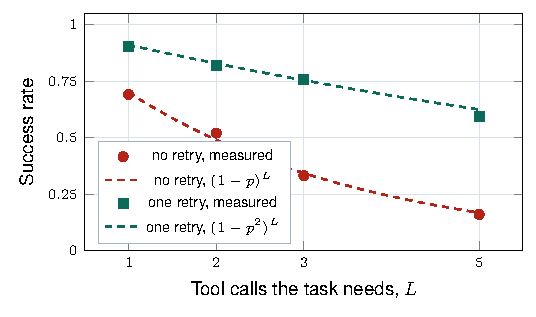
\includegraphics[width=\columnwidth]{length_plot.pdf}
\caption{Measured success against the closed-form expectation (\ref{eq:closed}) at
timeout rate 0.3, 200 trials per task.}
\label{fig:length}
\end{figure}

\subsection{Reliability Under Faults}
Table~\ref{tab:comparison} reports the three agents. Single-attempt success hides most
of the difference in dependability: one retry raises success from 0.58 to 0.77 but
pass$^5$ only from 0.25 to 0.33, while three retries reach 1.00 on both at about twice
the cost and latency of the naive agent. The paired test separates three retries from
one retry with 14 discordant runs, all favoring three retries ($p = 1.2 \times
10^{-4}$), and from no retry with 25 ($p = 6.0 \times 10^{-8}$). The diagnosis also
shows the price of retrying: twelve runs by the three-retry agent answered correctly but
exceeded their step budget and were flagged as horizon failures.

\begin{table}[t]
\caption{Agents Under 30\% Tool Timeouts (12 Tasks, 5 Trials)}
\label{tab:comparison}
\centering
\footnotesize
\setlength{\tabcolsep}{2.6pt}
\begin{tabular}{lccccc}
\toprule
\textbf{Agent} & \textbf{Success [95\% CI]} & \textbf{pass$^5$} & \textbf{Cost (\$)} & \textbf{Lat. (ms)} & \textbf{Root causes} \\
\midrule
naive & 0.58 [0.38, 0.77] & 0.25 & 0.0016 & 543 & 25 recovery \\
retry, 1 & 0.77 [0.67, 0.88] & 0.33 & 0.0025 & 947 & 14 recovery \\
retry, 3 & 1.00 [1.00, 1.00] & 1.00 & 0.0030 & 1116 & 12 horizon \\
\bottomrule
\end{tabular}
\end{table}

Fig.~\ref{fig:stress} sweeps the timeout rate from 0 to 0.5. The gap between success
and pass$^5$ widens with the fault rate for every agent, which is the inconsistency a
single attempt per task cannot reveal.

\begin{figure}[t]
\centering
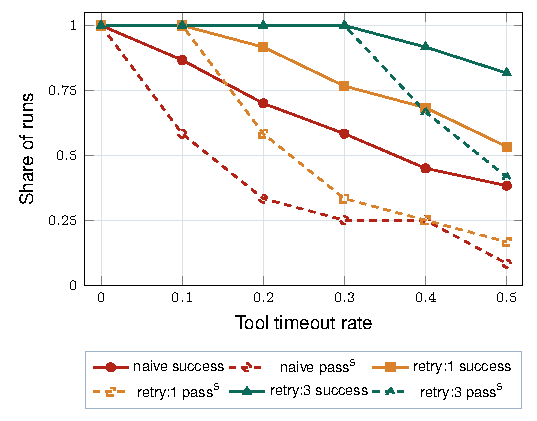
\includegraphics[width=\columnwidth]{stress_plot.pdf}
\caption{Success (solid) and pass$^5$ (dashed) as the tool timeout rate rises.}
\label{fig:stress}
\end{figure}

\subsection{The Classifier Recovers Planted Defects}
Each reference agent carries one planted defect: no retry, answering from memory,
repeating calls, or calling a forbidden tool, plus a retrying control agent.
Table~\ref{tab:selfcheck} counts the root cause diagnosed in each of 60 runs per agent.
Every diagnosed run of a planted agent is attributed to its planted mode, giving a
precision of 1.00 for all four modes. Runs counted as none are runs where the defect
never surfaced, for example a naive agent that met no timeout. The control agent shows
one genuine recovery failure, three consecutive timeouts on one call, and eleven
step-budget overruns.

\begin{table}[t]
\caption{Diagnosed Root Causes per Planted Defect (60 Runs Each)}
\label{tab:selfcheck}
\centering
\setlength{\tabcolsep}{3.5pt}
\begin{tabular}{llcccccc}
\toprule
\textbf{Agent} & \textbf{Planted} & \textbf{Plan.} & \textbf{Misuse} & \textbf{Ctx.} & \textbf{Recov.} & \textbf{Horiz.} & \textbf{None} \\
\midrule
naive & recovery & 0 & 0 & 0 & 25 & 0 & 35 \\
guessing & planning & 55 & 0 & 0 & 0 & 0 & 5 \\
looping & context & 0 & 0 & 55 & 0 & 0 & 5 \\
careless & misuse & 0 & 60 & 0 & 0 & 0 & 0 \\
retry & control & 0 & 0 & 0 & 1 & 11 & 48 \\
\bottomrule
\end{tabular}
\end{table}

\subsection{Choosing a Retry Budget}
A sweep over zero to four retries at a 0.3 timeout rate places every setting on the
Pareto front, because each extra retry buys success with cost and latency. Success rises
0.58, 0.77, 0.98, 1.00, and 1.00, with pass$^5$ of 0.25, 0.33, 0.92, 1.00, and 1.00.
For a target of 0.95 the recommendation is two retries, the cheapest setting that
meets it.

\subsection{Limitations}
The reference agents follow fixed tool plans, so these experiments test the instrument,
not the reasoning of LLMs. Tools are mock lookups, faults are limited to timeouts and
outages, and the rule-based classifier cannot judge the content of free-text reasoning.
The next phase runs hosted and local LLMs through the included adapter and adds suites
adapted from public benchmarks.

\section{Conclusion}

Agent Reliability Lab turns the question of whether an agent works into controlled
experiments on how consistently it works, why it fails, and what reliability costs.
Agent-independent fault schedules make variant comparisons paired, repeated trials
expose inconsistency that single attempts hide, and evidence-based diagnosis explains
each failure without inventing labels. Preliminary experiments confirm that the fault
injector matches its analytic expectation and that the classifier recovers planted
defects. Future work will evaluate live LLM agents, add fault kinds such as rate limits
and corrupted outputs, import traces from tracing platforms, and study whether the
taxonomy transfers to multi-agent systems.

\section*{Acknowledgment}

The authors thank Prof.\ Tripti Sharma, Head of the Department of Computer Science and
Engineering, Noida Institute of Engineering and Technology, Greater Noida, for her
guidance and support, and Mr.\ Pradeep Kumar, Assistant Professor, for his supervision
and technical feedback throughout this project.

\begin{thebibliography}{00}
\bibitem{yao2023react} S. Yao, J. Zhao, D. Yu, N. Du, I. Shafran, K. Narasimhan, and Y. Cao, ``ReAct: Synergizing reasoning and acting in language models,'' in \textit{Proc. Int. Conf. Learn. Represent. (ICLR)}, 2023.
\bibitem{liu2024agentbench} X. Liu \textit{et al.}, ``AgentBench: Evaluating LLMs as agents,'' in \textit{Proc. ICLR}, 2024.
\bibitem{mialon2024gaia} G. Mialon, C. Fourrier, C. Swift, T. Wolf, Y. LeCun, and T. Scialom, ``GAIA: A benchmark for general AI assistants,'' in \textit{Proc. ICLR}, 2024.
\bibitem{jimenez2024swebench} C. E. Jimenez, J. Yang, A. Wettig, S. Yao, K. Pei, O. Press, and K. Narasimhan, ``SWE-bench: Can language models resolve real-world GitHub issues?'' in \textit{Proc. ICLR}, 2024.
\bibitem{zhou2024webarena} S. Zhou \textit{et al.}, ``WebArena: A realistic web environment for building autonomous agents,'' in \textit{Proc. ICLR}, 2024.
\bibitem{yao2024taubench} S. Yao, N. Shinn, P. Razavi, and K. Narasimhan, ``$\tau$-bench: A benchmark for tool-agent-user interaction in real-world domains,'' arXiv:2406.12045, 2024.
\bibitem{barres2025tau2} V. Barres, H. Dong, S. Ray, X. Si, and K. Narasimhan, ``$\tau^2$-bench: Evaluating conversational agents in a dual-control environment,'' arXiv:2506.07982, 2025.
\bibitem{chen2021codex} M. Chen \textit{et al.}, ``Evaluating large language models trained on code,'' arXiv:2107.03374, 2021.
\bibitem{kapoor2024agents} S. Kapoor, B. Stroebl, Z. S. Siegel, N. Nadgir, and A. Narayanan, ``AI agents that matter,'' arXiv:2407.01502, 2024.
\bibitem{kapoor2026hal} S. Kapoor \textit{et al.}, ``Holistic agent leaderboard: The missing infrastructure for AI agent evaluation,'' in \textit{Proc. ICLR}, 2026.
\bibitem{rabanser2026reliability} S. Rabanser, S. Kapoor, P. Kirgis, K. Liu, S. Utpala, and A. Narayanan, ``Towards a science of AI agent reliability,'' in \textit{Proc. 43rd Int. Conf. Mach. Learn. (ICML)}, PMLR, vol. 306, 2026.
\bibitem{basiri2016chaos} A. Basiri, N. Behnam, R. de Rooij, L. Hochstein, L. Kosewski, J. Reynolds, and C. Rosenthal, ``Chaos engineering,'' \textit{IEEE Software}, vol. 33, no. 3, pp. 35--41, 2016.
\bibitem{ruan2024toolemu} Y. Ruan \textit{et al.}, ``Identifying the risks of LM agents with an LM-emulated sandbox,'' in \textit{Proc. ICLR}, 2024.
\bibitem{toolmisusebench2026} ``ToolMisuseBench: An offline deterministic benchmark for tool misuse and recovery in agentic systems,'' arXiv:2604.01508, 2026.
\bibitem{toolbenchx2026} ``Beyond function calling: Benchmarking tool-using agents under tool-environment unreliability,'' arXiv:2606.25819, 2026.
\bibitem{agentchaos2026} ``AgentChaos: Chaos engineering for agent systems via programmatic fault injection,'' arXiv:2608.06790, 2026.
\bibitem{cemri2025mast} M. Cemri \textit{et al.}, ``Why do multi-agent LLM systems fail?'' arXiv:2503.13657, 2025.
\bibitem{deshpande2025trail} D. Deshpande, V. Gangal, H. Mehta, J. Krishnan, A. Kannappan, and R. Qian, ``TRAIL: Trace reasoning and agentic issue localization,'' arXiv:2505.08638, 2025.
\bibitem{zhang2025whowhen} S. Zhang \textit{et al.}, ``Which agent causes task failures and when? On automated failure attribution of LLM multi-agent systems,'' in \textit{Proc. 42nd Int. Conf. Mach. Learn. (ICML)}, PMLR, vol. 267, 2025.
\bibitem{liang2023helm} P. Liang \textit{et al.}, ``Holistic evaluation of language models,'' \textit{Trans. Mach. Learn. Res.}, 2023.
\bibitem{inspect2024} UK AI Security Institute, ``Inspect: A framework for large language model evaluations,'' 2024. [Online]. Available: \url{https://inspect.aisi.org.uk}
\bibitem{wilson1927} E. B. Wilson, ``Probable inference, the law of succession, and statistical inference,'' \textit{J. Amer. Statist. Assoc.}, vol. 22, no. 158, pp. 209--212, 1927.
\bibitem{efron1979} B. Efron, ``Bootstrap methods: Another look at the jackknife,'' \textit{Ann. Statist.}, vol. 7, no. 1, pp. 1--26, 1979.
\bibitem{mcnemar1947} Q. McNemar, ``Note on the sampling error of the difference between correlated proportions or percentages,'' \textit{Psychometrika}, vol. 12, no. 2, pp. 153--157, 1947.
\bibitem{dietterich1998} T. G. Dietterich, ``Approximate statistical tests for comparing supervised classification learning algorithms,'' \textit{Neural Comput.}, vol. 10, no. 7, pp. 1895--1923, 1998.
\end{thebibliography}

\end{document}
